\chapter{Agrupamento}
Agrupamento é usar as características de entrada para descobrir aglomerações naturais nos dados e para dividir os dados nestes grupos \cite{real2013}. Ou ainda, particionar itens em regiões homogêneas. Um exemplo aplicado a redes sociais é: encontrar comunidades dentro de um grande grupo de pessoas \cite{foundations2012}.

Dentre os algoritmos mais conhecidos de agrupamento estão: K-médias, modelos de mistura gaussianas e clusterização hierárquicas. Um dos métodos mais interessantes para realizar agrupamento é o SOM (Self Organizing Map, Mapa auto-organizável) desenvolvido por Teuvo Kohonen em 1982 \cite{kohonen1982}. Além de realizar o agrupamento com robustez, o SOM é capaz de operar uma redução de dimensionalidade nos dados, dessa forma não somente a morfologia dos agrupamentos é interessante, mas também o mapa gerado pelo algoritmo. Entretanto este algoritmo ainda apresenta o modelo de lote, possuindo fase de treino e uso bem distintas.

\section{SOM}
É possível pensar o algoritmo SOM como uma combinação de dois sistemas menores. Uma parte funciona como uma rede neural competitiva do tipo o vencedor leva tudo. Nesta etapa um dos neurônios da rede é selecionado de acordo com sua semelhança a amostra de entrada, este neurônio é o único vencedor daquela amostra. O segundo sistema acontece depois que o neurônio é escolhido, agora a rede irá se adaptar para incorporar esse novo aprendizado, o peso do neurônio vencedor e de seus vizinhos é alterado, isto é o que dá plasticidade à rede. 
De acordo com Teuvo em \citeonline{kohonen1982} o processo auto-organizável do algoritmo pode ser simplificado em quatro etapas:

\begin{enumerate}
\item Um vetor de unidades de processamento que recebem estímulos coerentes de um espaço de eventos e formam funções discriminantes simples com base nas entradas.
\item Um mecanismo que compara as funções discriminantes e seleciona a unidade que possui o maior valor.
\item Algum tipo de interação local, que, simultaneamente, ativa a unidade vencedora e seus vizinhos.
\item Um processo adaptativo que faz os parâmetros das unidades ativadas aumentarem seus valores de função discriminante com base na atual entrada.
\end{enumerate}

Na figura 12 pode-se observar a arquitetura de mapa auto-organizado. As variáveis \textit{epsilon} representam as entradas do sistema, elas são comparadas com todas as unidades de processamento \textit{eta}, e o neurônio que for mais parecido é o vencedor daquela amostra. As unidades de processamento também possuem o conceito de vizinhança, quanto mais próximos uma unidade for da outra, mais parecidas elas serão. A redução de dimensionalidade é alcançada pois, ao fim do treinamento, cada unidade de processamento será um represente do conjunto de entradas que ele foi capaz de selecionar. A figura 13 demonstra a saída de uma rede SOM aplicada a um conjunto de cores, é possível observar que a rede foi capaz de reduzir a dimensionalidade e as características semelhantes ficaram próximas umas das outras.    

\begin{figure}[!h]
\centering
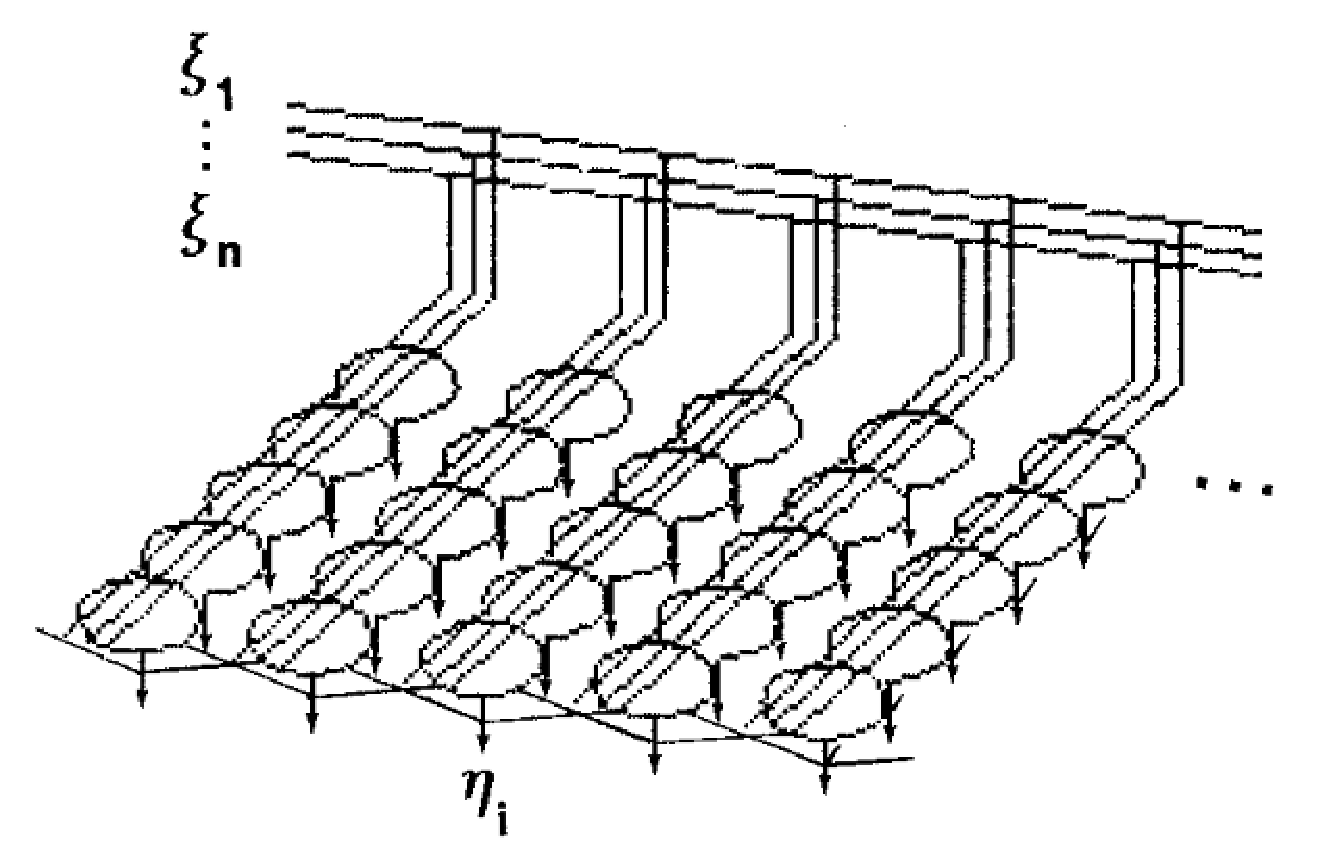
\includegraphics[keepaspectratio=true,scale=0.40]
{figuras/redesom.eps}
\caption{Sistema que Apresenta um Mapa Organizado - \cite{kohonen1982}}
\label{data_titatic}
\end{figure}


\begin{figure}[!h]
\centering
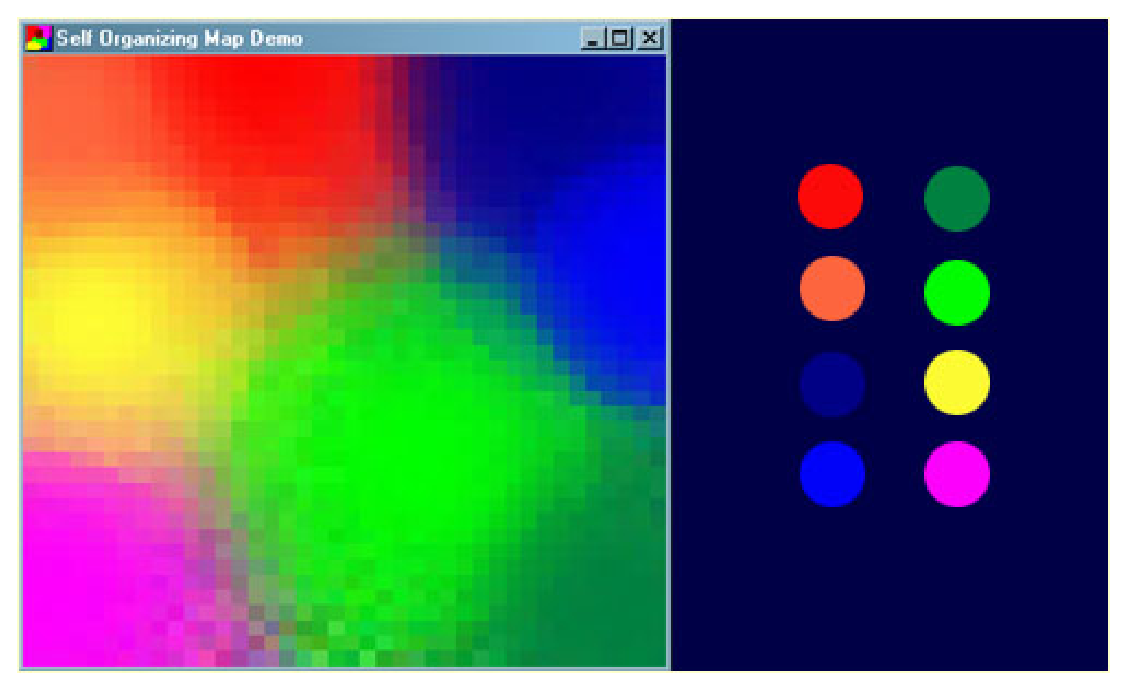
\includegraphics[keepaspectratio=true,scale=0.50]
{figuras/dimensionreduction.eps}
\caption{Exemplo de Redução de Dimensionalidade - \cite{somaijk}}
\label{data_titatic}
\end{figure}

A aplicação SOM pode ser separada em duas etapas, treino e uso. Na etapa de treino as entradas são apresentadas, selecionadas e os parâmetros do mapa são ajustados para incorporar o aprendizado. O processo de treino ocorre até que uma de três condições sejam alcançadas. Ou a quantidade de épocas de treino é atingida, ou o taxa de aprendizado chegue a zero ou a rede atinja algum critério de erro pré-estabelecido que seja aceitável. A etapa de uso é uma variação do treino, as amostras de entrada são apresentadas ao sistema e alguma unidade de processamento será capaz de selecioná-la, a diferença desta etapa para o treino é que não há nenhum aprendizado ou ajuste de parâmetro. O SOM é incapaz de aprender continuamente, pois seus parâmetros internos decaem com tempo, chegando a estabilidade total, onde não há mais aprendizado.

    




 










